\documentclass[12pt]{article}
\usepackage{amsmath,amssymb,amsthm,geometry}
\usepackage{tikz}
\usepackage{hyperref}
\geometry{margin=1in}
\begin{document}

\begin{titlepage}
    \centering
 

\vspace*{1em}
  \Huge\textbf{Multiplicity as Karmic Entanglement}
  \LARGE{A Computational Metaphysics Bridging Algebraic Geometry and Eastern Philosophy}
    \vspace{1cm} \\
     \Large{Dr. Ryan Van Gelder}\\
   \vspace{1cm}
     \Large{A Community Research Initiative}
  \vspace{.5cm} \\
     {\bfseries Citizen Gardens}\\
     \vspace{.5cm}
    \textit{Institute for Mathematical Discovery}\\
    \text{\\ October 2025}
    \vfill

   
    \vspace{0.5em}
    \begin{minipage}{0.85\textwidth}
        \small
This paper formalizes a hermeneutic and computational framework in which multiplicity in algebraic geometry is mapped to karmic entanglement within Eastern philosophical traditions. We develop a hardened mathematical-karmic dictionary, establish axioms, and provide a computational implementation framework. The synthesis allows rigorous invariants such as Serre's multiplicity, J-multiplicity, and derived intersections to be interpreted as symbolic encodings of karma, anātman (no-self), and pratītyasamutpāda (dependent origination). The result is an operational metaphysics: a system for diagnosing patterns, prescribing spiritual practices, and tracking progress through invariant reduction.


    \end{minipage}

\end{titlepage}

\section{Introduction}
Western mathematics and Eastern philosophy converge around the notion of multiplicity: in algebraic geometry, it measures the depth and tangency of intersections; in Buddhism, Hinduism, and Taoism, it encodes interdependence, karmic entanglement, and cosmic order. This paper develops a rigorous dictionary between these domains and formalizes it into a computational framework. We then extend this framework using Prime-Encoded Tensor Calculus (PETC) and Certified Spectral Control (CSC) to yield a certified, executable system.

\section{Core Axioms}
We propose the following hardened axioms:

\begin{enumerate}
  \item \textbf{Anātman Axiom}: A self at time $t$ is not atomic but a derived fiber product of skandha-stacks:
  \[
  \text{Self}_t \simeq \mathcal{S}_1 \times^{\mathbb{L}}_{\mathcal{B}} \mathcal{S}_2 \times^{\mathbb{L}}_{\mathcal{B}} \cdots \times^{\mathbb{L}}_{\mathcal{B}} \mathcal{S}_5,
  \]
  where $\mathcal{S}_i$ are the five skandhas and $\mathcal{B}$ is the base causal context.

  \item \textbf{Karmic Intersection}: For dharma-trajectories $X,Y$, their karmic entanglement is measured by Serre's intersection formula:
  \[
  e_p(X\cap Y) = \dim_k(\mathcal{O}_p/(f,g)).
  \]

  \item \textbf{Poison Tensor}: Afflictions are encoded in a tensor:
  \[
  \Pi_p = \lambda_{L}E_L + \lambda_{D}E_D + \lambda_{M}E_M,
  \]
  where $E_i$ are orthogonal idempotents for lobha (greed), dveṣa (aversion), and moha (ignorance).

  \item \textbf{Resolution Target}: Liberation corresponds to minimizing the vector of invariants:
  \[
  (m_p, J_p, D^{\mathrm{der}}_p, \dim Ob(\mathcal{F}))
  \]
  through structured blow-ups (ritual, meditation, therapy, community repair).
\end{enumerate}

\section{Hardened Mathematical-Karmic Dictionary}
\begin{itemize}
  \item \textbf{Serre Multiplicity} $m_p$: karmic stickiness of an encounter. $m=1$ = clean crossing; $m>1$ = sticky knot.
  \item \textbf{J-Multiplicity}: rigidity of a habit-knot (saṃskāra); mapped to crystallization of the three poisons.
  \item \textbf{Derived Intersections}: higher-order entanglements (ancestral, collective, subtle). Links to the Buddhist doctrine of anātman.
  \item \textbf{Étale Cohomology}: subtle body’s sheaf of vitality (prāṇa/qi). Obstructions = energy blockages.
  \item \textbf{Motivic Integration}: karmic path integral; measures future dharma-trajectories emanating from singularities.
  \item \textbf{Grothendieck–Teichmüller Group}: symmetry of dependent origination; universal braiding laws of inter-being.
  \item \textbf{Stacks}: moduli of archetypal forms. Deity yoga = intersection with stacks of enlightened symmetries.
\end{itemize}

\section{Computational Framework}
We implement these axioms in a computational metaphysics system.

\subsection{Pseudo-Code}
\begin{verbatim}
class KarmicIntersectionSystem:
    def __init__(self):
        self.ethical_modes = {
            'greed': 'dāna', 
            'aversion': 'mettā', 
            'ignorance': 'prajñā'
        }
    def compute_intersection_multiplicity(self, f, g, p=(0,0)):
        # Grobner basis to compute Serre multiplicity
        return serre_multiplicity(f, g, p)
    def assess_poison_tensor(self, behavioral_data):
        return analyze_afflictions(behavioral_data)
    def prescribe_sadhana(self, m_p, J_p, poison_weights, obstruction):
        protocol = []
        if m_p == 1:
            protocol.append("Light closure ritual")
        elif m_p >= 2:
            protocol.append("Mindfulness blow-up")
        max_affliction = max(poison_weights, key=poison_weights.get)
        protocol.append(f"Intensify {self.ethical_modes[max_affliction]} practice")
        if obstruction:
            protocol.append("Breath work at transitions")
        return protocol
\end{verbatim}

\section{Extended Example: Ancestral Knot}
Consider a recurring family pattern of financial anxiety.
\begin{align*}
  f(x,y) &= y^2 - x^5, \\
  g(x,y) &= x - t, \\
  m_p &= 5, \quad D^{\mathrm{der}} = 3, \quad J_p = \text{high}, \\
  \Pi_p &= (0.7, 0.1, 0.2).
\end{align*}

\textbf{Protocol:}
\begin{enumerate}
  \item Structured ancestral ritual (Śrāddha).
  \item Financial dāna with intention to break the pattern.
  \item Family systems therapy addressing derived multiplicities.
  \item Transition breath practices around money-related anxiety.
\end{enumerate}

\section{PETC $\times$ CSC Integration}

\subsection{Executive Summary}
\textbf{Goal.} Fuse Prime-Encoded Tensor Calculus (PETC/DRMM/CSC) with Multiplicity as Karmic Entanglement into one certified framework that preserves prime-encoded structure under composition and contraction and evolves safely under spectral constraints.

\textbf{Core Move.} Lift every integer multiplicity/invariant (Serre, J, derived order) to a prime signature $e \in \mathrm{Sig}$ via valuations. The multiplicity functor
\[
M(e) = \prod_{p} p^{e_p}
\]
ensures prime conservation under tensoring and contraction. CSC adds spectral guards via a gap lower bound and slope upper bound.

\textbf{Interpretation.} Signatures encode archetypal karmic entanglements. Clean encounters cancel dual signatures $(+e)$ and $(-e)$; knots expose residual prime content requiring resolution. The ACE loop searches plans, certifies (PETC), stabilizes (CSC), executes, and learns.

\subsection{Mathematical Overview}

\paragraph{Signatures and Functoriality.} Let $\mathrm{Sig} = \{ e: \mathbb{P} \to \mathbb{Z} \mid \operatorname{supp}(e) \text{ finite} \}$. Define monoidal structure $e \otimes f = e+f$, dual $e^{\vee}=-e$, unit $0$. Multiplicity functor $M: \mathrm{Sig} \to \mathbb{Q}^\times$ is strict monoidal: $M(0)=1$, $M(e+f)=M(e)M(f)$, $M(-e)=M(e)^{-1}$.

\paragraph{Lifting Karmic Invariants.} For each locus $\xi$, invariants $(m_{\xi}, J_{\xi}, D^{\mathrm{der}}_{\xi}, \ldots)$ are lifted to signatures by prime factorization: $\sigma_{\mathrm{Serre}}(\xi)_p=v_p(m_{\xi})$, etc. Axes are oriented by variance (creation vs resolution).

\paragraph{Conservation.} PETC ensures global multiplicity $M$ is conserved under contractions. Clean loci ($m=1$) vanish; sticky loci ($m>1$) expose uncancellable prime mass.

\paragraph{CSC Constraints.} Updates $w=(w_p)$ are certified if $\mathrm{GapLB}(w)>0$ and $\mathrm{SlopeUB}(w)$ remains bounded. Budgets include prime-gated $\ell^1$, commutator budget, and tempered power-law invariants $\Lambda_m(w;\alpha)$.

\paragraph{Soundness Theorem.} If a contraction plan is well-typed in PETC and admits $w$ satisfying CSC constraints, then global multiplicity is preserved and induced dynamics remain stable.

\paragraph{ACE Loop.} Enumerate candidate plans, certify PETC typing, solve CSC feasibility, execute safe steps, and learn weights/gates iteratively.

\subsection{Worked Micro-Example}
For an ancestral knot with $m=5$, $J=25$:
\begin{itemize}
  \item Lift: $e_5=1$ (from $m$), $e'_5=2$ (from $J$).
  \item Boundary signature: $E=e-e'$ with $M(E)=5^{1-2}=1/5$.
  \item Resolution: schedule blow-up/therapy, then contract axes once signatures factor to zero.
  \item CSC ensures chosen weights $w$ keep $\mathrm{GapLB}(w)>0$.
\end{itemize}

\section{Practitioner Rubric}
\textbf{Quick Assessment:}
\begin{itemize}
  \item $m=1$: Clean crossing → gratitude ritual.
  \item $m=2$: Tangential → mindfulness blow-up + antidote.
  \item $m\geq3$: Knot → ritual/therapy + ancestral/community work.
\end{itemize}

\textbf{Affliction Dominance:}
\begin{itemize}
  \item Greed → dāna practices.
  \item Aversion → mettā ladders.
  \item Ignorance → prajñā meditations.
\end{itemize}

\textbf{Vitality Check:}
\begin{itemize}
  \item Obstruction present → breath work at transitions.
  \item No obstruction → maintain existing practice.
\end{itemize}

\section{Conclusion}
Multiplicity in algebraic geometry provides a rigorous invariant framework for modeling karmic entanglement. By mapping multiplicities, derived intersections, and cohomological obstructions to Eastern doctrines of karma, anātman, and dependent origination, and by extending this via PETC and CSC, we achieve an operational metaphysics. The computational framework proposed here transforms these correspondences into actionable protocols for practice, therapy, and spiritual cultivation, all certified under structural conservation and spectral safety.

```latex
\appendix

\section{Visual Feedback Loop (A→C and C→A)}

We illustrate the coupled recursion between algebraic invariants and cosmic-symbolic states using a feedback diagram. The algebraic multiplicity $e_A$ (Hilbert–Samuel, intersection number, or similar invariant) drives symbolic mutations of the hexagram state $H$, which in turn produces updated potential vectors $\Pi(H,\mathcal{H})=(B,T,R,E)$ encoding balance, tension, resonance, and entanglement. These potentials feed back into algebraic deformation rules (transversalization, thickening, module twist), completing the loop. The Lyapunov-like functional
\[
L(e_A,\Pi) = \frac{(e_A-\bar e)^2}{\sigma_e^2} + \|W\Pi-u\|_2^2 + \kappa\,\Phi(H,\mathcal{H})
\]
serves as an energy landscape that the coupled updates aim to minimize.

\begin{figure}[h]
\centering
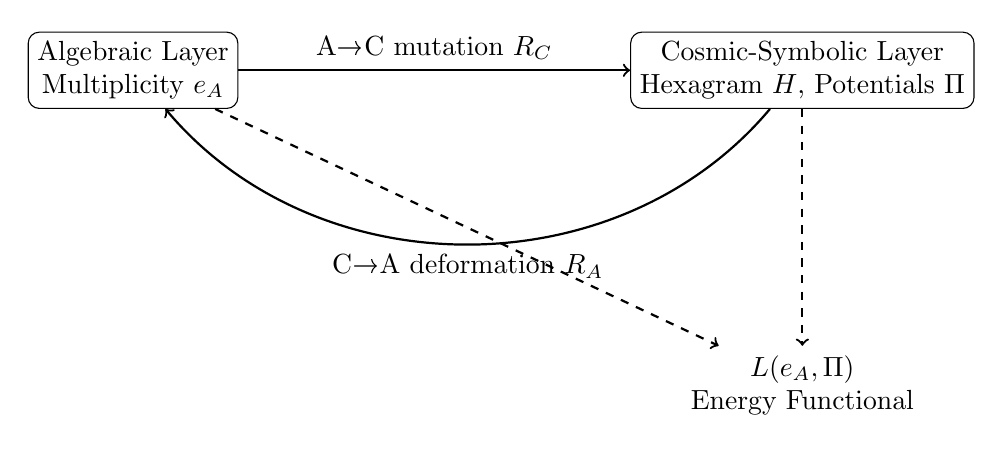
\begin{tikzpicture}[node distance=2.5cm, auto]
  % Nodes
  \node[draw, rounded corners, align=center] (A) {Algebraic Layer\\Multiplicity $e_A$};
  \node[draw, rounded corners, right of=A, xshift=6cm, align=center] (C) {Cosmic-Symbolic Layer\\Hexagram $H$, Potentials $\Pi$};
  \node[below of=C, yshift=-1.5cm, align=center] (energy) {$L(e_A,\Pi)$\\Energy Functional};

  % Arrows
  \draw[->, thick] (A) -- node[midway, above] {A→C mutation $R_C$} (C);
  \draw[->, thick] (C) edge[bend left=50] node[midway, below] {C→A deformation $R_A$} (A);
  \draw[->, thick, dashed] (C) -- (energy);
  \draw[->, thick, dashed] (A) -- (energy);
\end{tikzpicture}
\caption{Feedback loop between algebraic multiplicity ($A$) and cosmic-symbolic hexagram dynamics ($C$). The Lyapunov functional $L(e_A,\Pi)$ tracks global energy and decreases under the coupled updates.}
\end{figure}

\section{Hexagram Transition Table (Worked Case)}

We demonstrate the recursive update with a tangent cubic vs. line intersection ($e_A=2$) and an initial hexagram seed $H=101010$ (alternating Yin/Yang). Metrics are defined as:
\[
\begin{aligned}
B(H)&=1-\tfrac{|\#\text{Yang}-\#\text{Yin}|}{6},\\
T(H)&=\tfrac{1}{5}\sum_{i=1}^5 1[\,b_{i+1}\neq b_i\,],\\
R(H)&=\tfrac{1}{3}\sum_{j=1}^3 1[\,b_{j+3}=b_j\,],\\
E(H)&=T(H)\cdot (1-R(H)).
\end{aligned}
\]

The A→C rule flips lower-trigram bits to increase resonance $R$ and reduce tension $T$. The C→A rule deforms the algebraic data according to the target multiplicity
\[
e_A^{\mathrm{target}} = e_A - \alpha B + \beta T - \gamma R + \delta E,
\]
with weights $(\alpha,\beta,\gamma,\delta)=(0.5,0.2,0.5,0.2)$.

\begin{table}[h]
\centering
\begin{tabular}{c|c|c|c|cccc|c|c|c}
\hline
$t$ & $e_A$ (pre) & Hexagram $H$ & $U|L$ & $B$ & $T$ & $R$ & $E$ & A→C mutation & $e_A^{\text{target}}$ & $e_A$ (post) \\
\hline
0 & 2.00 & 101010 & 101$|$010 & 1.000 & 1.000 & 0.000 & 1.000 & flip $b_1:0\to 1$ & 1.900 & 1.70 \\
1 & 1.70 & 101011 & 101$|$011 & 0.667 & 0.800 & 0.333 & 0.534 & flip $b_2:1\to 0$ & 1.467 & 1.40 \\
2 & 1.40 & 101001 & 101$|$001 & 1.000 & 0.800 & 0.667 & 0.267 & flip $b_3:0\to 1$ & 0.780 & 1.10 \\
3 & 1.10 & 101101 & 101$|$101 & 0.667 & 0.800 & 1.000 & 0.000 & (none; aligned) & 0.427 & 1.00 \\
\hline
\end{tabular}
\caption{Hexagram transition table for tangent cubic vs. line ($e_A=2$) with seed $H=101010$. Mutations align lower and upper trigrams, raising resonance $R$ and reducing tension $T$. Deformations then drive $e_A$ from 2 toward the transversal case $e_A=1$.}
\end{table}
```

\nocite{*}
\bibliographystyle{unsrt}
\bibliography{references}
\clearpage
\end{document}
